\section{Monday for MAT4002}\index{Monday_lecture}
\subsection{Quotient Map}
\begin{definition}[Quotient Map]\label{def:7:6}
A mapping $q:X\to Y$ between topological spaces is a \emph{quotient map} if 
\begin{enumerate}
\item
$q$ is surjective
\item
For any $U\subseteq Y$, $U$ is open iff $q^{-1}(U)$ is open.
\end{enumerate}
\end{definition}
\begin{remark}
\begin{enumerate}
\item
The canonical projection mapping $p:X\to X/\sim$ is a quotient mapping
\item
We say $f$ is an open mapping if $U$ is open in $X$ implies $f(U)$ is open in $Y$.
Note that a continuous open mapping satisfies condition~(2) in definition~(\ref{def:7:6}).
\end{enumerate}
\end{remark}

In proposition~(\ref{pro:6:5}) we show the homeomorphism between $X/\sim$ and $Y$ given the compactness of $X$ and Hausdorffness of $Y$.
Now we show the homeomorphism by replacing these conditions with the quotient mapping $q$:

\begin{proposition}
Suppose $q:X\to Y$ is a quotient map, and that $\sim$ is an equivalence relation on $X$ given by the partition $\{q^{-1}(y)\mid y\in Y\}$.
Then $X/\sim$ and $Y$ are \emph{homeomorphic}.
\end{proposition}
\begin{proof}
Construct the mapping 
\[
\begin{array}{ll}
h:&X/\sim\to Y\\
\text{with}&h([x]) = q(x)
\end{array}
\]
Note that:
\begin{enumerate}
\item
The mapping $h$ is well-defined and injective.
\item
Surjective is easy to shown.
\item
The quotient mapping $q:=h\circ p$, by definition, is continuous.
By applying proposition~(\ref{pro:6:4}), $h$ is continuous.
\end{enumerate}
It suffices to show $h^{-1}$ is continuous:
\begin{itemize}
\item
For any open $\tilde{U}\subseteq X/\sim$, it suffices to show $h(\tilde{U})$ is open in $Y$.

Note that
\[
q^{-1}(h(\tilde{U}))=p^{-1}h^{-1}(h(\tilde{U}))=p^{-1}(\tilde{U}),
\]
which is open by the definition of quotient topology~(check proposition~(\ref{pro:6:1})).

Therefore, $h(\tilde U)$ is open by (2) in definition~(\ref{def:7:6}).
\end{itemize}
\end{proof}

\begin{example}
The $\mathbb{R}/\mathbb{Z}$ is homeomorphic to the unit circle $S^1$:

Define the mapping
\[
\begin{array}{ll}
q:&\mathbb{R}\to S^1\\
&x\mapsto e^{2\pi i x}
\end{array}
\]
It's clear that
\begin{enumerate}
\item
$q$ is a continuous open mapping~(why?)
\item
$q$ is surjective
\end{enumerate}
Therefore, $\mathbb{R}/\sim\cong S^1$, provided that $x\sim y$ iff $q(x)=q(y)$, i.e., $x-y\in\mathbb{Z}$.
Therefore, 
\[
\mathbb{R}/\mathbb{Z}\cong S^1
\]
\end{example}


\subsection{Simplicial Complex}
\begin{quotation}
Combinatorics is the slums of topology.\qquad\quad---~J. H. C. Whitehead
\end{quotation}
The idea is to build some new spaces from some ``fundamental'' objects.
The combinatorialists often study topology by the combinatorics of these fundamental objects.
First we define what are the ``fundamental'' objects:

\begin{definition}[$n$-simplex]
The standard $n$-simplex is the set
\[
\Delta^n = \left\{(x_1,\dots,x_{n+1})\in\mathbb{R}^{n+1}\middle| x_i\ge0,\forall i\text{ and } \sum_{i=1}^{n+1}x_i=1\right\}
\]
\begin{figure}[H]
\centering
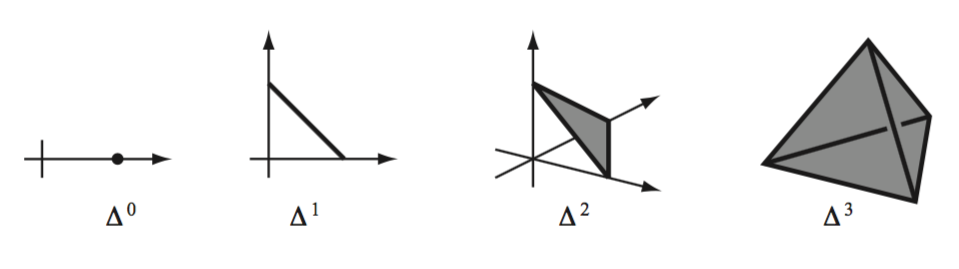
\includegraphics[width=0.6\textwidth]{week7/p_2}
\caption{Simplices on $\mathbb{R}^2$ are the triangles, so you may consider simplexes as the ``triangles'' in general spaces}
\end{figure}
\begin{enumerate}
\item
The non-negative integer $n$ is the \emph{dimension} of this simplex
\item
Its \emph{vertices}, denoted as $V(\Delta^n)$, are those points $(x_1,\dots,x_{n+1})$ in $\Delta^n$ such that $x_i=1$ for some $i$.
\item
For each given non-empty $\mathcal{A}\subseteq\{1,\dots,n+1\}$, its \emph{face} is defined as
\[
\{(x_1,\dots,x_{n+1})\in\Delta^n\mid x_i=0,\ \forall i\notin\mathcal{A}\}
\]
In particular, $\Delta^n$ is a face of itself
\item
The \emph{inside} of $\Delta^n$ is
\[
\text{inside}(\Delta^n):=\{(x_1,\dots,x_{n+1})\in\Delta^n\mid x_i>0,\forall i\}
\]
In particular, the inside of $\Delta^0$ is $\Delta^0$.
\end{enumerate}
\end{definition}

\begin{definition}[Face Inclusion]
A face inclusion of $\Delta^m$ into $\Delta^n$ ($m<n$) is a function 
$\Delta^m\to\Delta^n$ which comes from the restriction of an \emph{injective linear} map
$f:\mathbb{R}^{m+1}\to\mathbb{R}^{n+1}$ that maps vertices in $\Delta^m$ into vertices in $\Delta^n$.
\end{definition}
For example, the linear transformation $f:\mathbb{R}^2\to\mathbb{R}^3$ defined below is a face inclusion:
\[
\begin{array}{ll}
f(1,0)=(0,1,0),
&
f(0,1)=(0,0,1).
\end{array}
\]
\begin{remark}
Any injection mapping from $\{1,\dots,m+1\}\to\{1,\dots,n+1\}$ gives a face inclusion $\Delta^m\to\Delta^n$, and vice versa.
\end{remark}

\paragraph{Motivation}
Now we build new spaces by making use of simplices.
This new space is called the \emph{abstract complex}.
If a simplex is a part of the complex, so are all its faces.

\begin{definition}[Abstract Simplicial Complex]
An (abstract) \emph{simplicial complex} is a pair $K=(V,\Sigma)$,
where $V$ is a set of vertices and $\Sigma$ is a collection of non-empty finite subsets of $V$ (simplices) such that
\begin{enumerate}
\item
For any $\bm v\in V$, the 1-element set $\{\bm v\}$ is in $\Sigma$
\item
If $\sigma$ is an element of $\Sigma$, then so is any non-empty subset of $\sigma$.
\end{enumerate}
\end{definition}
For example, if $V=\{1,2,3,4\}$, then
\[
\Sigma=\{\{1\},\{2\},\{3\},\{4\},\{1,3,4\},\{2,4\},\{1,3\},\{3,4\},\{1,4\}\}
\]

We can associate to an abstract simplicial complex $K$ a topological space $|K|$, which is called its \emph{geometric realization}:
\begin{definition}[Topological Realization]
The \emph{topological realization} of $K=(V,\Sigma)$ is 
a topological space $|K|$ (or denoted as $|(V,\Sigma)|$), where
\begin{enumerate}
\item
For each $\sigma\in\Sigma$ with $|\sigma|=n+1$, 
take a copy of $n$-simplex and denote it as $\Delta_\sigma$
\item
Whenever $\sigma\subset\tau\in\Sigma$, identify $\Delta_{\sigma}$ with a face of $\Delta_{\tau}$ through face inclusion.
\end{enumerate}
\end{definition}
\begin{remark}
Or equivalently, $|K|$ is a quotient space of the disjoint union
\[
\coprod _{\sigma\in\Sigma}\sigma
\]
by the equivalence relation which identifies a point $y\in\sigma$ with its image under the face inclusion $\sigma\to\tau$, for any $\sigma\subset\tau$.
\end{remark}




\begin{example}
Take 
\begin{figure}[H]
\centering
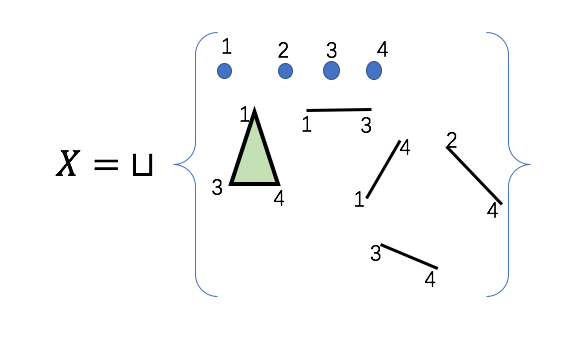
\includegraphics[width=0.6\textwidth]{week7/p_4}
\end{figure}
As a result, 
\begin{figure}[H]
\centering
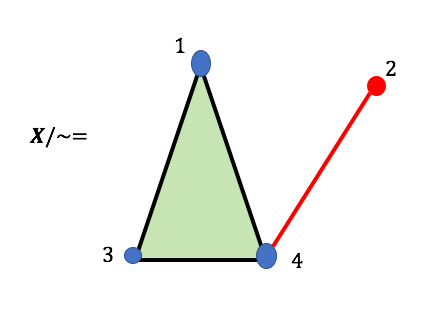
\includegraphics[width=0.6\textwidth]{week7/p_5}
\end{figure}
\end{example}

\begin{example}
Take $V=\{1,2,3,4\}$ and 
\[
\Sigma=\{\text{all subsets of $V$ except $V$}\}
\]
As shown in the figure below, $|(V,\Sigma)| = \Delta^3$:
\begin{figure}[H]
\centering
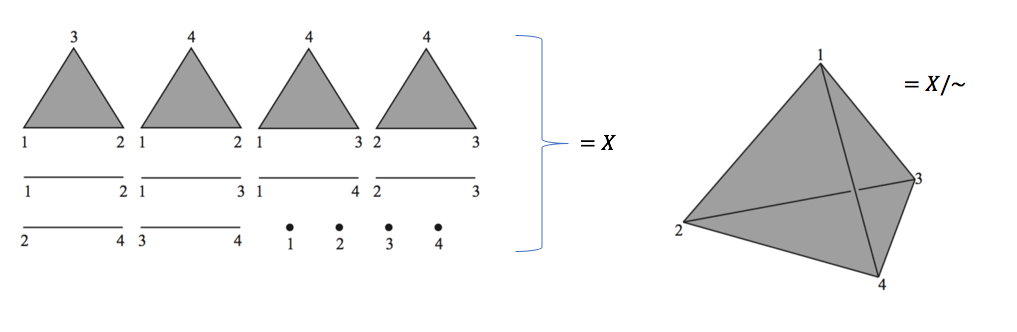
\includegraphics[width=\textwidth]{week7/p_7}
\end{figure}
\end{example}
%\begin{example}
%Take $V=\{1,\dots,n+1\}$ and
%\[
%\Sigma=\{\text{All subsets of $V$}\}
%\]
%Then $|(V,\Sigma)| = \Delta^n$.
%\end{example}

\begin{definition}[Triangulation]
A \emph{triangulation} of a topological space $X$ is a simplicial complex $K=(V,\Sigma)$ together with a choice of homeomorphism $|K|\to X$.
\end{definition}

\begin{example}
The triangulation of $S^1\times S^1$ can be realized by using nine vertices given below:
\begin{figure}[H]
\centering
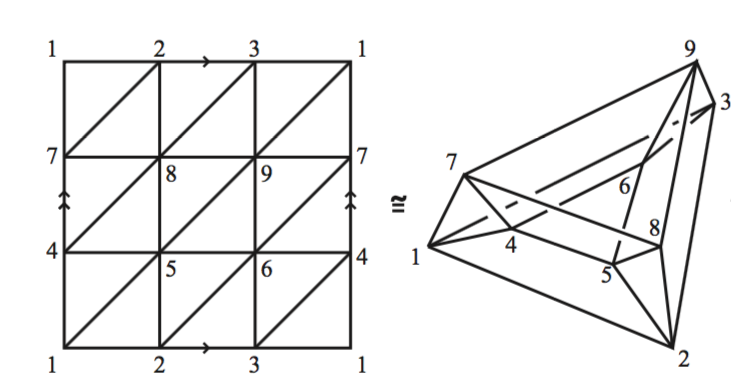
\includegraphics[width=0.7\textwidth]{week7/p_8}
\caption{The quotient space $|K|:=X/\sim$}
\end{figure}
(Try to identify $X$)
\end{example}



















